% PressSens_AoATracking.tex

\tikzstyle{EllipseObject}=[ultra thick, draw=blue, ellipse, minimum width=12em,
    minimum height=5em,align=center]
\tikzstyle{LabelObject}=[fill=white,rectangle,rounded corners,line width=0.5mm,%
	align=center]
\tikzstyle{ArrowObject}=[red,line width=1.0mm, -latex]

\resizebox{!}{0.45\textwidth}{
	\begin{tikzpicture}
		\node[anchor=south west,inner sep=0] (image) at (0,0)%
			{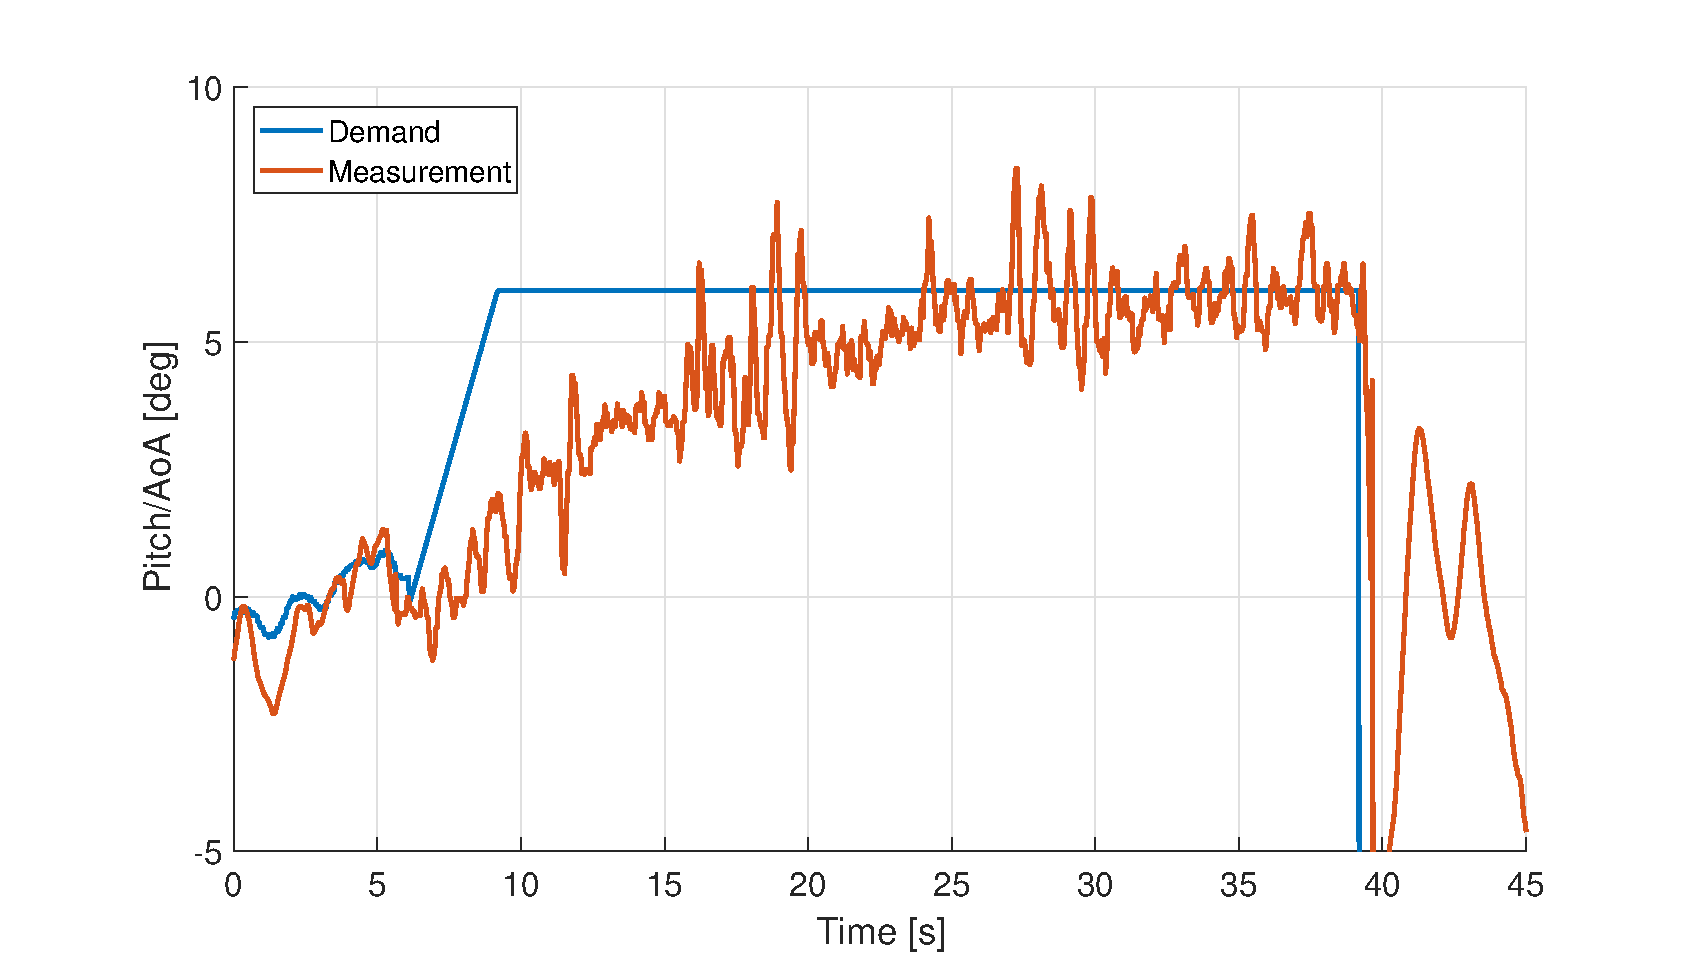
\includegraphics[width=\textwidth]{PressSens_AoATracking.eps}};
		% Define scope with 'image' dimensions as reference
		\begin{scope}[x={(image.south east)},y={(image.north west)}]
			%\draw[help lines,xstep=.05,ystep=.05] (0,0) grid (1,1);
			%\foreach \x in {0,1,...,9} { \node [anchor=north] at (\x/10,0) {0.\x}; }
			%\foreach \y in {0,1,...,9} { \node [anchor=east] at (0,\y/10) {0.\y}; }
			
			\only<9>{
			  % Active-Control node
			  \node at (0.24,0.4) (CtrlAct) {};
			  % Active-Control label
			  \draw(0.6,0.2) node[LabelObject] (CtrlAct_Label) {Control\\Activated};
			  % Active-Control arrow
			  \draw[ArrowObject] (CtrlAct_Label.west) -- (CtrlAct);
			}
			\only<10>{
			  % AoA-tracking node
			  \draw(0.6,0.7) node (AoATrack_Node) {};
			  % AoA-tracking marker
			  \node[EllipseObject] (AoATrack) at (AoATrack_Node) {};
			  % AoA-tracking label
			  \draw(0.4,0.2) node[LabelObject] (AoATrack_Label) {AoA\\Tracked!};
			  % AoA-tracking arrow
			  \draw[ArrowObject] (AoATrack_Label.north east) -- (AoATrack);
			}
			
		\end{scope}
  \end{tikzpicture}
}